\renewcommand{\a}{\vec{a}}
\renewcommand{\b}{\vec{b}}
\renewcommand{\p}{\vec{p}}
\renewcommand{\vector}[1]{\begin{bmatrix}#1\end{bmatrix}}



Notes on Classical Mechanics by John R. Taylor\footnote{http://www.amazon.com/Classical-Mechanics-John-R-Taylor/dp/189138922X}


\section{Newton's Laws of Motion}






\subsection{Basics}

The basic object of interest is a moving particle. Its position at time $t$ is
$\r$. It has that arrow over it because it is a vector. A vector is something
that specifies a direction and a magnitude. Think of $\r$ as an arrow from the
origin pointing to the current position. Don't think of $\r$ yet as a column
vector containing numbers, because we haven't said what coordinate system we're
using. Regardless of what coordinate system we use, $\r$ is always a vector
pointing from the origin to the current position.

The particle is moving, i.e. the position changes over time. So instead of just
writing $\r$, we write $\r(t)$ which says that it's a function of time. Think
of that as giving the answer to a question: "At a given time $t$, what is the
position?". The answer (position) is a vector, so we can say that this is a
"vector-valued function" (i.e. whatever output it gives, it's always a vector).

Its velocity is a function $\v(t)$ whose value is also a vector (at time $t$
it's going at some speed in some direction). The velocity function $\v(t)$ is
the derivative with respect to time of the position function $\r(t)$. That
sounds very familiar, but what exactly is the derivative of a vector-valued
function?

In normal, non-vector, calculus we imagine some curve like $y = x^2$. So $y$ is
a function of $x$. The value of that function is not a vector; it's just a
number (a scalar). The derivative of that function with respect to $x$ is
saying: at a particular point along the x-axis, if I start advancing $x$ a tiny
bit, how fast is $y$ changing? So, it's the slope of the curve at that point
(also just a number, not a vector).

In vector calculus, the derivative of $\r(t)$ with respect to $t$ is saying: at
some particular time $t$, if I start advancing time a tiny bit, where is the
position going and how fast is it going there? So the derivative of a
vector-valued function is a vector -- an arrow with direction and magnitude
(speed).


\subsection{Coordinate systems}

Thinking of $\r(t)$ as an arrow with direction and magnitude is correct but a
bit abstract. How specifically do we use numbers to represent position? The
chapter covers two main coordinate systems. Let's say the particle is moving in
2D space for now.

- \textbf{Cartesian coordinates}: we write down how far the particle currently is in
the x-direction, $x(t)$, and how far it currently is in the y-direction,
$y(t)$.

- \textbf{Polar coordinates}: we write down how far the particle currently is,
$r(t)$, in the current direction to the particle.

Note that $x(t)$, $y(t)$, and $r(t)$ were not written with arrows. They are
just numbers, saying how far the particle is *in some direction*. The "in some
direction" part corresponds to the concept of a *unit vector*. A "unit vector"
is basically a vector where the direction is of interest, but the magnitude is
just set to 1 for convenience.

Cartesian coordinates use two directions to specify the position. We'll write
these directions as the unit vectors $\xhat$ and $\yhat$. So in Cartesian
coordinates, the position is


\begin{align*}
  \r(t) = x(t)\xhat + y(t)\yhat
\end{align*}

(Go $x(t)$ units in the  $\xhat$ direction and $y(t)$ units in the $\yhat$ direction.)


In contrast, polar coordinates just use one direction to specify the position: the direction of a
direct line to the particle's current position. This direction is the unit vector $\rhat(t)$. So in
polar coordinates, the position is

\begin{align*}
\r(t) = r(t)\rhat(t)
\end{align*}

(Go $r(t)$ units in the $\rhat(t)$ direction)


Notice (and this is pretty important; it's basically the reason the chapter is
covering polar coordinates) that in polar coordinates the unit vector
$\rhat(t)$ is a function of time (its direction changes as the particle moves);
in contrast, in Cartesian coordinates, $\xhat$ and $\yhat$ are constant; they
always point in the same direction. The polar unit vector is a function of time
because it is the direction to wherever-the-particle-currently-is. The
Cartesian unit vectors are not functions of time because they are just the
x-axis direction and the y-axis direction and these do not change.

\subsection{Velocity}


We can now differentiate these position functions to get the velocity. Recall
that the answer is going to be a vector because it is the derivative of a
vector-valued function.

\textbf{Cartesian coordinates}

Because $\xhat$ and $\yhat$ are not functions of time, differentiating is
straightforward:

\begin{align*}
\v(t) = \frac{d}{dt}\bigg(x(t)\xhat + y(t)\yhat\bigg) = \frac{d x(t)}{dt}\xhat + \frac{d y(t)}{dt} \yhat
\end{align*}

Physicists use a dot to represent derivative-with-respect-to-time. So they
might write this as

\begin{align*}
\v(t) =  \dot x(t) \xhat + \dot y(t) \yhat
\end{align*}

Either way, what this is saying is that in Cartesian coordinates, the velocity
function is a vector comprised of current x-speed in the x-direction and
current y-speed in the y-direction. In other words, it's what you expect.

\textbf{Polar coordinates}

\begin{align*}
\v(t) = \frac{d}{dt}\bigg(r(t)\rhat(t)\bigg)
\end{align*}

That's a product of two things that are both a function of time, so we use the
"product rule"[ref] The product rule is the thing when you studied
differentiation that says: when you're differentiating the product of two
functions you differentiate one and keep the other as-is, then you
differentiate the other while keeping the first as-is, and you add the two
things together: $\frac{d(f(t)g(t))}{dt} = \dot f(t) g(t) + f(t) \dot g(t)$
[/ref] to differentiate it:

\begin{align*}
\frac{d}{dt}\bigg(r(t)\rhat(t)\bigg) = \dot r(t) \rhat(t) + r(t)\frac{d \rhat(t)}{dt}
\end{align*}

There's quite a few $r$s there and it's important at this stage not to get lost in the symbols. We
know that the answer (velocity) is a vector. That means we can write it as a bunch of things added
together, where each thing is a number times some unit vector. And we're using polar coordinates, so
the unit vectors are going to be the polar unit vectors. So the thing on the left
$\dot r(t) \rhat(t)$ is fine: that's saying that the velocity has one component which is the current
radial speed (a number $\dot r(t)$) in the current radial direction (the unit vector $\rhat(t)$).

What about the thing on the right? It's the current radial distance times the
current derivative of the unit vector function. We've said that in polar
coordinates the unit vector $\rhat(t)$ changes over time, so it does make sense
that we could ask what its derivative with respect to time is. So what is it?
The answer is that it's a vector-valued function whose current value always
points at right-angles to the current radial direction, but that requires
explaining:

Going back to the informal definition of derivatives above, we're at some point
$t$ in time, and we imagine starting to advance time a tiny bit, and we look at
the change in where the unit vector points, after this infinitesimally small
amount of time passes. A unit vector always has length 1, so it can't grow in
length. There's only one thing it can do: it can point in a slightly different
direction. What direction has it gone in? It's basically like the hand of a
clock. It's not too hard to see that if the hand of a clock changes just a tiny
bit, then the tip moves in a direction that's almost a tangent to the
circle. Change "tiny" to "infinitesimally small" and the "almost" goes away: so
the time derivative of the radial unit vector is a vector pointing at right
angles to the radial vector. This unit vector in that direction is called
$\phihat$, because it points in the direction that you go in when you increase
the angle $\phi$, as opposed to $\rhat$ which points in the direction you go in
if you increase the radius $r$. How fast does the radial unit vector move in
the $\phihat$ direction? The answer is that it moves at the speed that the
angle is increasing, so $\dot \phi$[ref]You can prove this by writing the unit
vector in Cartesian coordinates, $cos(\phi) \xhat + sin(\phi) \yhat$, and then
differentiating it to give $\dot \phi\big(-sin(\phi)\xhat +
cos(\phi)\yhat\big)$ which is $\dot \phi$ times a vector orthogonal to the
original one.[/ref]. In other words, the time derivative of the radial unit
vector is $\dot \phi(t) \phihat(t)$

The conclusion of all that is that in polar coordinates, the velocity vector is

\begin{align*}
\v(t) = \dot r(t) \rhat(t) + r(t) \dot \phi(t) \phihat(t)
\end{align*}

Compare this with the expression for velocity in Cartesian coordinates

\begin{align*}
\v(t) =  \dot x(t) \xhat + \dot y(t) \yhat
\end{align*}

and we see it's a bit more complicated in polar coordinates.

I understand the polar coordinates version as follows. At time $t$ the particle
might be moving radially, and its angle might also be changing. The velocity
vector has two components, one in the radial direction, and one in the tangent
direction. In the radial direction, it's moving at whatever speed the radius is
changing with. In the tangent direction it's moving at the speed that the angle
is changing, multiplied by the current radius. That multiplication by radius
makes sense informally, because if you are further out from the center of a
circle, and the circle rotates by a few degrees, then you move further in space
than if you were closer in to the center.


\subsection{Acceleration}


The acceleration function is the derivative of the velocity function with
respect to time. Therefore, it is also a vector: at time $t$ the particle is
accelerating by some amount, in some direction.

\textbf{Cartesian coordinates}

Again, because the unit vectors do not change with time, it's as you expect:
there's an x-acceleration in the x-direction, and a y-acceleration in the
y-direction.

\begin{align*}
\a(t) = \ddot x(t) \xhat + \ddot y(t) \yhat
\end{align*}

\textbf{Polar coordinates}

Above we saw that because, in polar coordinates, the directions of the
coordinate system change with time, the function for velocity was more
complicated than when using Cartesian coordinates. For acceleration, we
differentiate the velocity expression and of course it gets even more
complicated. But basically the answer is still a function of the form

\begin{align*}
\a(t) = \bigg( \text{Some function of } t \bigg) \rhat(t) + \bigg( \text{Another function of } t \bigg) \phihat(t)
\end{align*}

The functions of $t$ involve the current radius length, the speed and
acceleration in the current radius direction, and the speed and acceleration of
the angle parameter $\phi$. The full expression is in the footnote[ref]In polar
coordinates, if you suppose that you know functions $r(t)$ and $\phi(t)$ giving
the angle and distance at time $t$, then the accelerations in the two
orthogonal directions at time $t$ are
$\a(t) = \bigg( \ddot r(t) - r(t) \dot\phi(t)^2 \bigg) \rhat(t) + \bigg( 2\dot r(t) \dot \phi(t) + r(t) \ddot \phi(t)\bigg) \phihat(t)$
[/ref].


\subsection{Newton's second law as a differential equation}

A key point seems to be: view Newton's second law $\F = m\a$ as a differential
equation[ref]The dot means "differentiated with respect to time". So if $r$ is
position as a function of time then $\dot r$ is velocity and $\ddot r$ is
acceleration.[/ref]:

\begin{align*}
m \ddot \r(t) = \F
\end{align*}

I'm understanding this as follows: You know what forces are acting on the body
in question. You want to know how the position of the body will evolve through
time: $\r(t)$. This is a function satisfying the following differential
equation: the second derivative with respect to time of $\r(t)$, times $m$, is
equal to the net force acting on the body.

In practice: in a typical problem you have some expression for $\F$ derived from
consideration of a diagram showing forces acting on the body. You might be able
to discover $\r(t)$ by finding a function whose second derivative is $\F$.

\subsection{Example problems}

\textbf{Cartesian coordinates}

> 1.37 A student kicks a frictionless puck with initial speed $v_0$, so that it
> slides up a plane that is inclined at an angle $\theta$ above the
> horizontal. \textbf{(a)} Write down Newton's second law for the puck and solve to
> give its position as a function of time.

This is a simple example of using the Second Law as a differential equation. We
write down the forces acting on the particle, set them equal to $m\ddot r(t)$
and integrate twice to get position.

The only force acting on the puck is its weight, i.e. its mass times
acceleration due to gravity: $mg$. The puck can only move along the surface of
the plane, so we are only interested in the component of the force that acts
parallel to the plane. This component is $-mg sin(\theta)$. So taking $x$ as the
direction up the plane, Newton's second law is

\begin{align*}
 m\ddot x(t) = -mgsin(\theta)
\end{align*}

Integrating once gives velocity

\begin{align*}
 \dot x(t) = -g sin(\theta) t + v_0
\end{align*}

Integrating again gives position

\begin{align*}
 x(t) = -\frac{1}{2} g sin(\theta) t^2 + v_0t + x_0
\end{align*}

and $x_0=0$ since we start measuring from its starting position.

> \textbf{(b)} How long will the puck take to return to its starting point?

The puck is at its starting point whenever $x = 0$:

\begin{align*}
0 = t\bigg(-\frac{1}{2} g sin(\theta) t + v_0\bigg)
\end{align*}

The solutions of that are either $t=0$ (which we already knew) or (the solution
we want)

$t = \frac{2v_0}{g sin(\theta)}$

\textbf{Polar coordinates}

> A "halfpipe" at a skateboard park consists of a concrete trough with a
> semicircular cross section of radius $R = 5m$. I hold a frictionless
> skateboard on the side of the trough pointing down toward the bottom and
> release it. Discuss the subsequent motion using Newton's second law. In
> particular, if I release the skateboard just a short way from the bottom, how
> long will it take to come back to the point of release?

Conceptually, we do the same thing as for the problem using Cartesian
coordinates: we write down Newton's second law resolved into two orthogonal
directions. It's just that with polar coordinates, these orthogonal directions
are constantly changing.

The weight of the skateboard acts downwards. This results in a tangent force
causing the skateboard to move along the halfpipe, and also presses the
skateboard into the halfpipe a bit, with an associated reaction force. We
ignore the force/reaction force between the skateboard and the pipe and focus
only on the tangent force: $-mg sin(\phi)$.

The equation for acceleration says that, at time $t$, acceleration in the
current tangent direction is $R\ddot \phi(t)$ (halfpipe radius times current
angular acceleration[ref]To see this, start with the $\phihat(t)$ (tangent
direction) part of the full expression for acceleration and note that the
radial distance of the skateboard is fixed by the presence of the half-pipe, so
speed $\dot r(t)$ (and acceleration) in the radial direction is
zero.[/ref]). So Newton's second law in this context is the differential
equation

\begin{align*}
mR \ddot \phi(t) = -mg sin(\phi(t))
\end{align*}

We read this as saying:

> We don't know how the angle is changing over time $\phi(t)$ -- that is
> precisely what we want to know. But what we do know is that whatever that
> function is, its second derivative at time $t$ is equal to the sin of the
> current angle (times $g/R$ and with a minus sign because the way we've
> defined the angle it gets smaller as the weight force takes the skateboard
> towards the bottom).

Once we've got to that point, finding the angle function $\phi(t)$ is just
math. It turns out that the only function for which it is true that the second
derivative has this property[ref]Actually the solution is a function with
second derivative having a different property, but one which is very similar to
the desired property as long as we're restricting ourselves to the angle being
fairly small.[/ref] is


\begin{align*}
  \phi(t) = \phi_0 cos\bigg(\sqrt\frac{g}{R}t\bigg)
\end{align*}

where $\phi_0$ is the angle that the skateboard was released at at time $t=0$.
This is the "solution" of the differential equation: a function matching the
criteria that the differential equation specified.

So we have our answer: the forces acting on the skateboard imply (via Newton's
second law) that the way the angle of the skateboard changes is a cosine
function of time. So the skateboard angle does what cosines do: it starts off
at its maximum, decreases to zero, crosses zero and becomes negative for a
while, starts turning back towards zero, crosses zero and becomes positive
again and gets back to its maximum where it turns around again.


\subsection{Conservation of momentum}

Momentum is mass times velocity, $\p(t) = m\dot \r(t)$, so another way of
stating the second law is: rate of change of momentum is equal to force. In a
multi-particle system the forces-and-reaction-forces of the third law cancel
each other out when summing the rate of change of momentum of the whole
system. So, total momentum doesn't change due to internal forces (but it does
if there are external forces).

pp 21-23 show that conservation of momentum does not hold when considering
magnetic and electrostatic forces between charged particles moving close to the
speed of light. However I am unfamiliar with those forces and with the
"right-hand rule" for fields/forces and I haven't understood this section.


\section{Work, energy}

\begin{mdframed}
  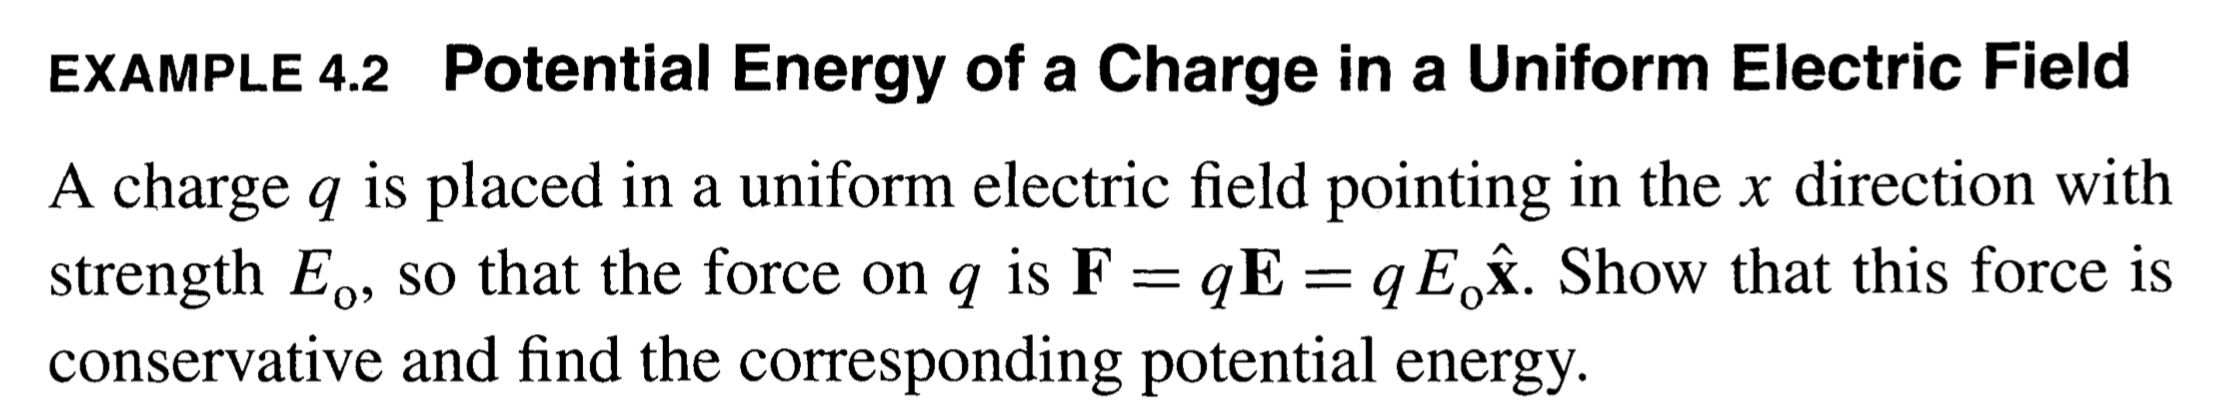
\includegraphics[width=400pt]{img/physics--classical-mechanics--taylor--ex-4-2.png}
\end{mdframed}

The components of the force are given by $\F(\r) = (F_x, F_y, F_z) = (qE_0, 0, 0)$.

To show that the force is conservative we must show
\begin{enumerate}
\item That it depends on no variable other than position.
  \begin{proof}
    The force is constant (doesn't even vary with position).
  \end{proof}

\item That the work done when moving between two positions does not depend on the path.
  \begin{proof}
    Let $\r_0$ and $\r_1$ be two positions and let $S$ be a path joining them. Then
    \begin{align*}
      W(\r_0 \to \r_1)
      &= \int_S \F(\r) \cdot \d \r \\
      &= qE_0\int_S \xhat \d\r \\
      &= qE_0\int_S 1 \dx \\
      &= qE_0(x_1 - x_0).
    \end{align*}
    Therefore the work depends only on the endpoints $x_0$ and $x_1$.
  \end{proof}
  The potential energy relative to $x_0, y_0, z_0$ is
  \begin{align*}
    V(x, y, z) = -qE_0(x - x_0).
  \end{align*}
\end{enumerate}



\begin{mdframed}
  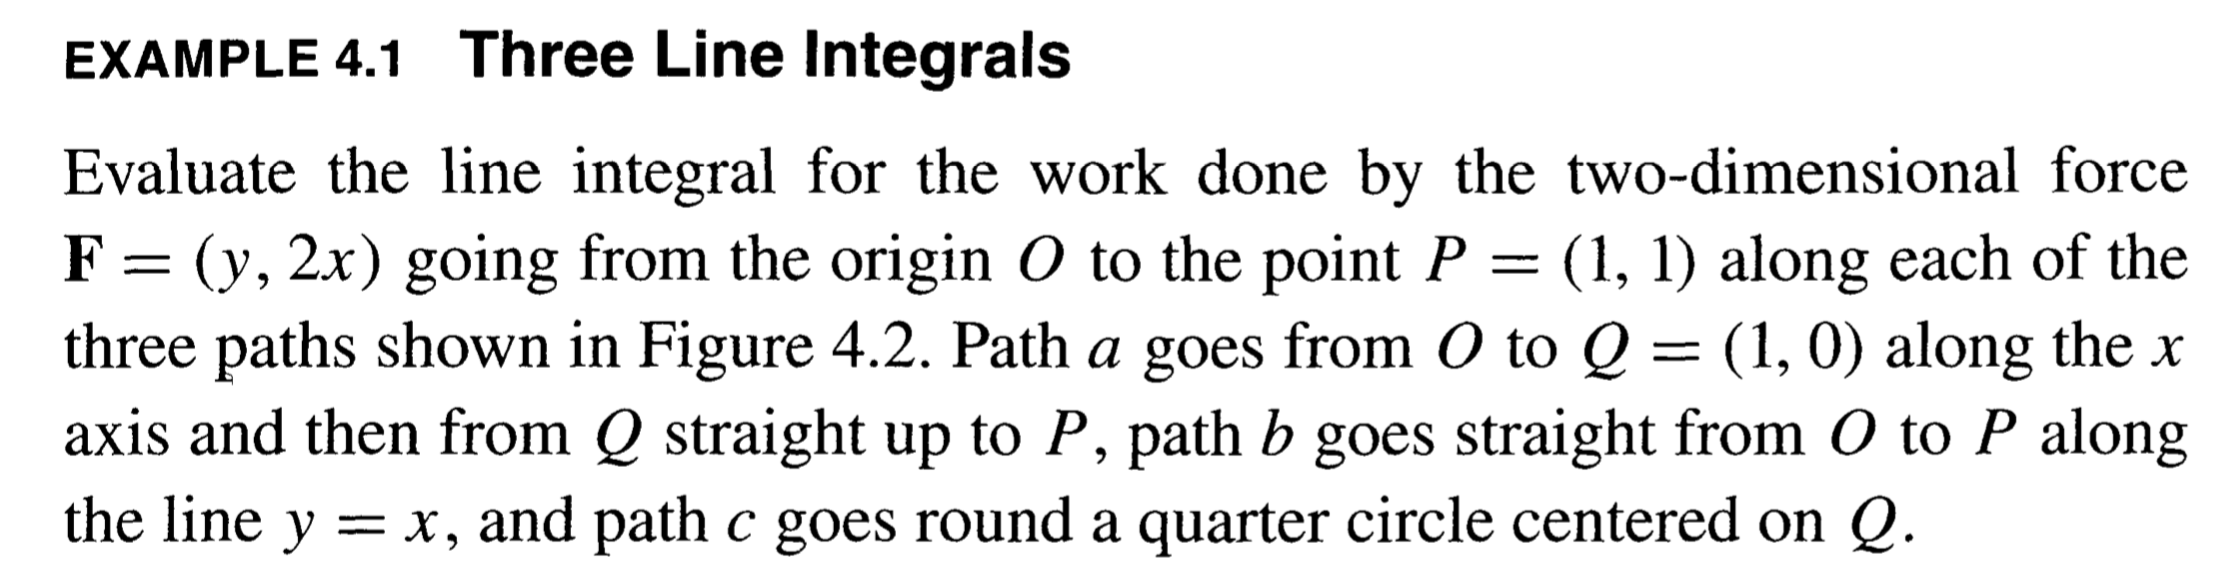
\includegraphics[width=400pt]{img/physics--classical-mechanics--taylor--ex-4-1.png}\\
  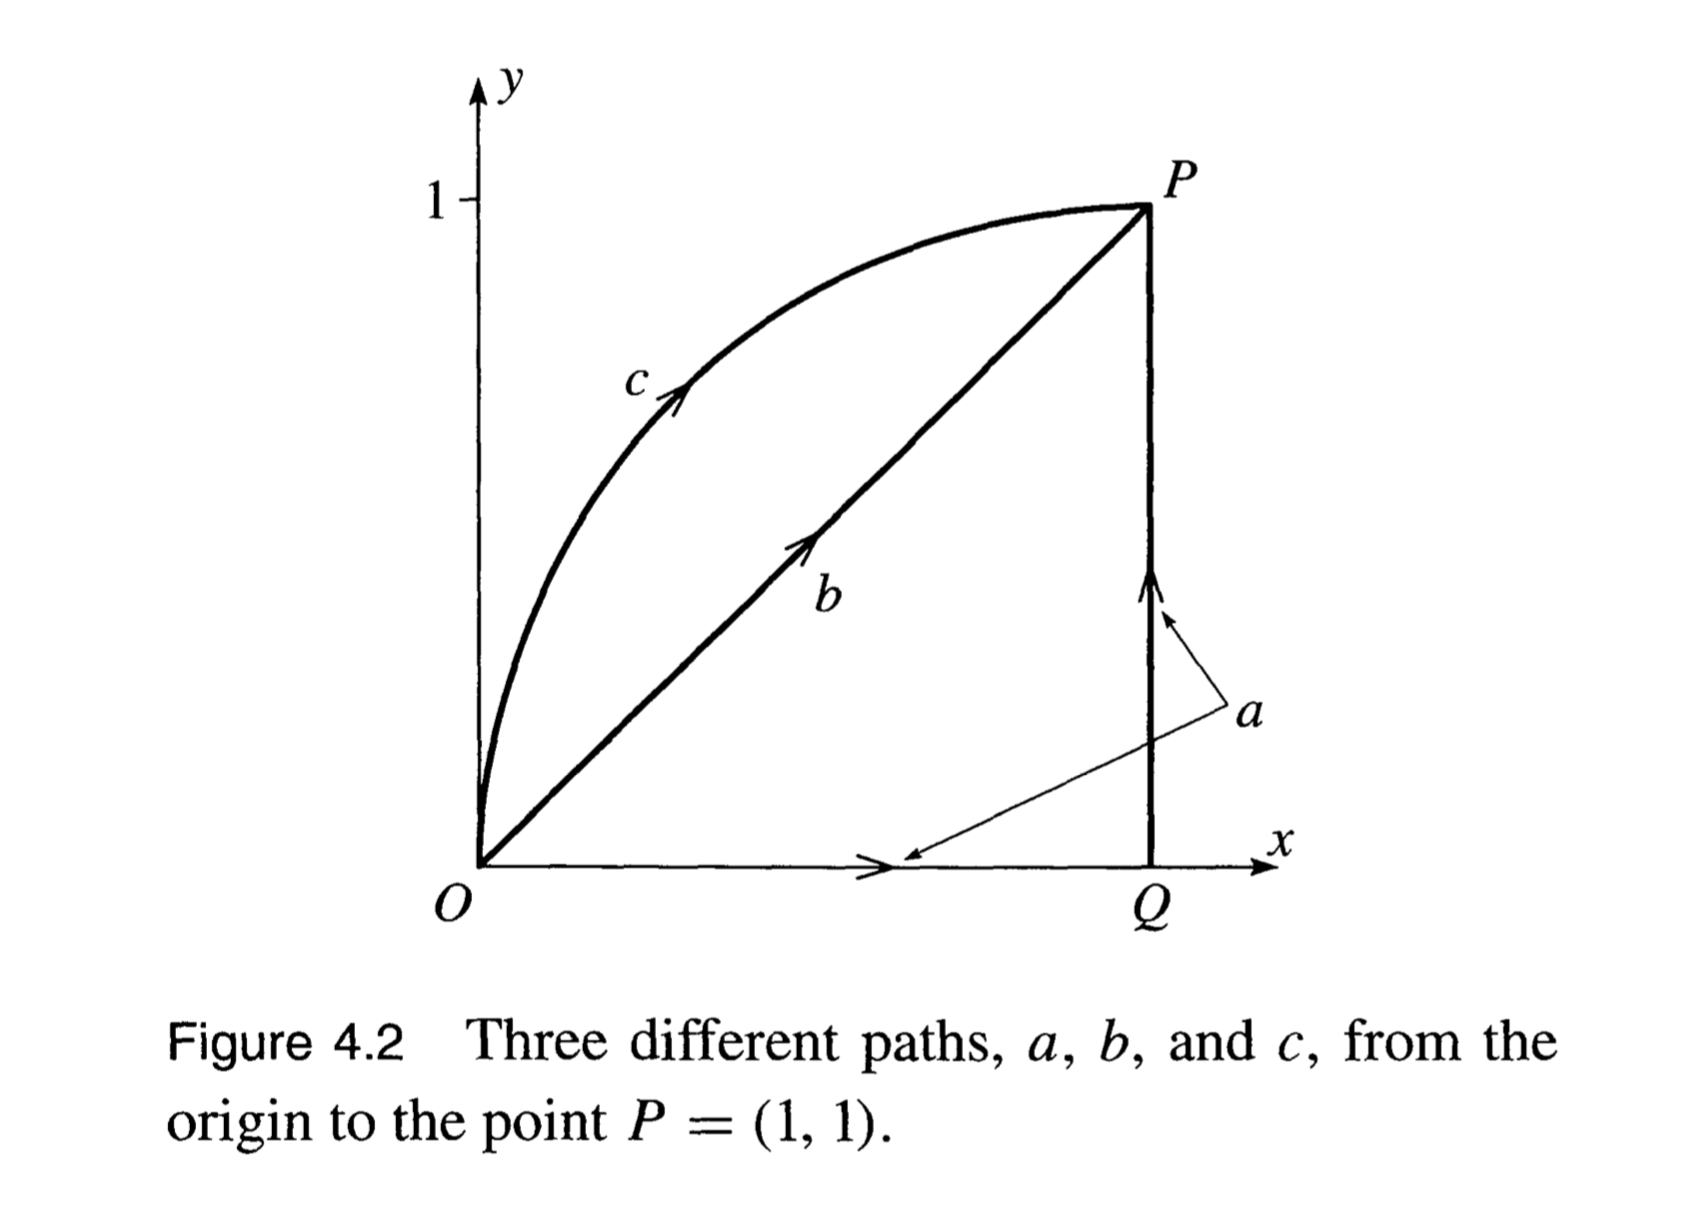
\includegraphics[width=200pt]{img/physics--classical-mechanics--taylor--ex-4-1-diag.png}
\end{mdframed}
\begin{mdframed}
  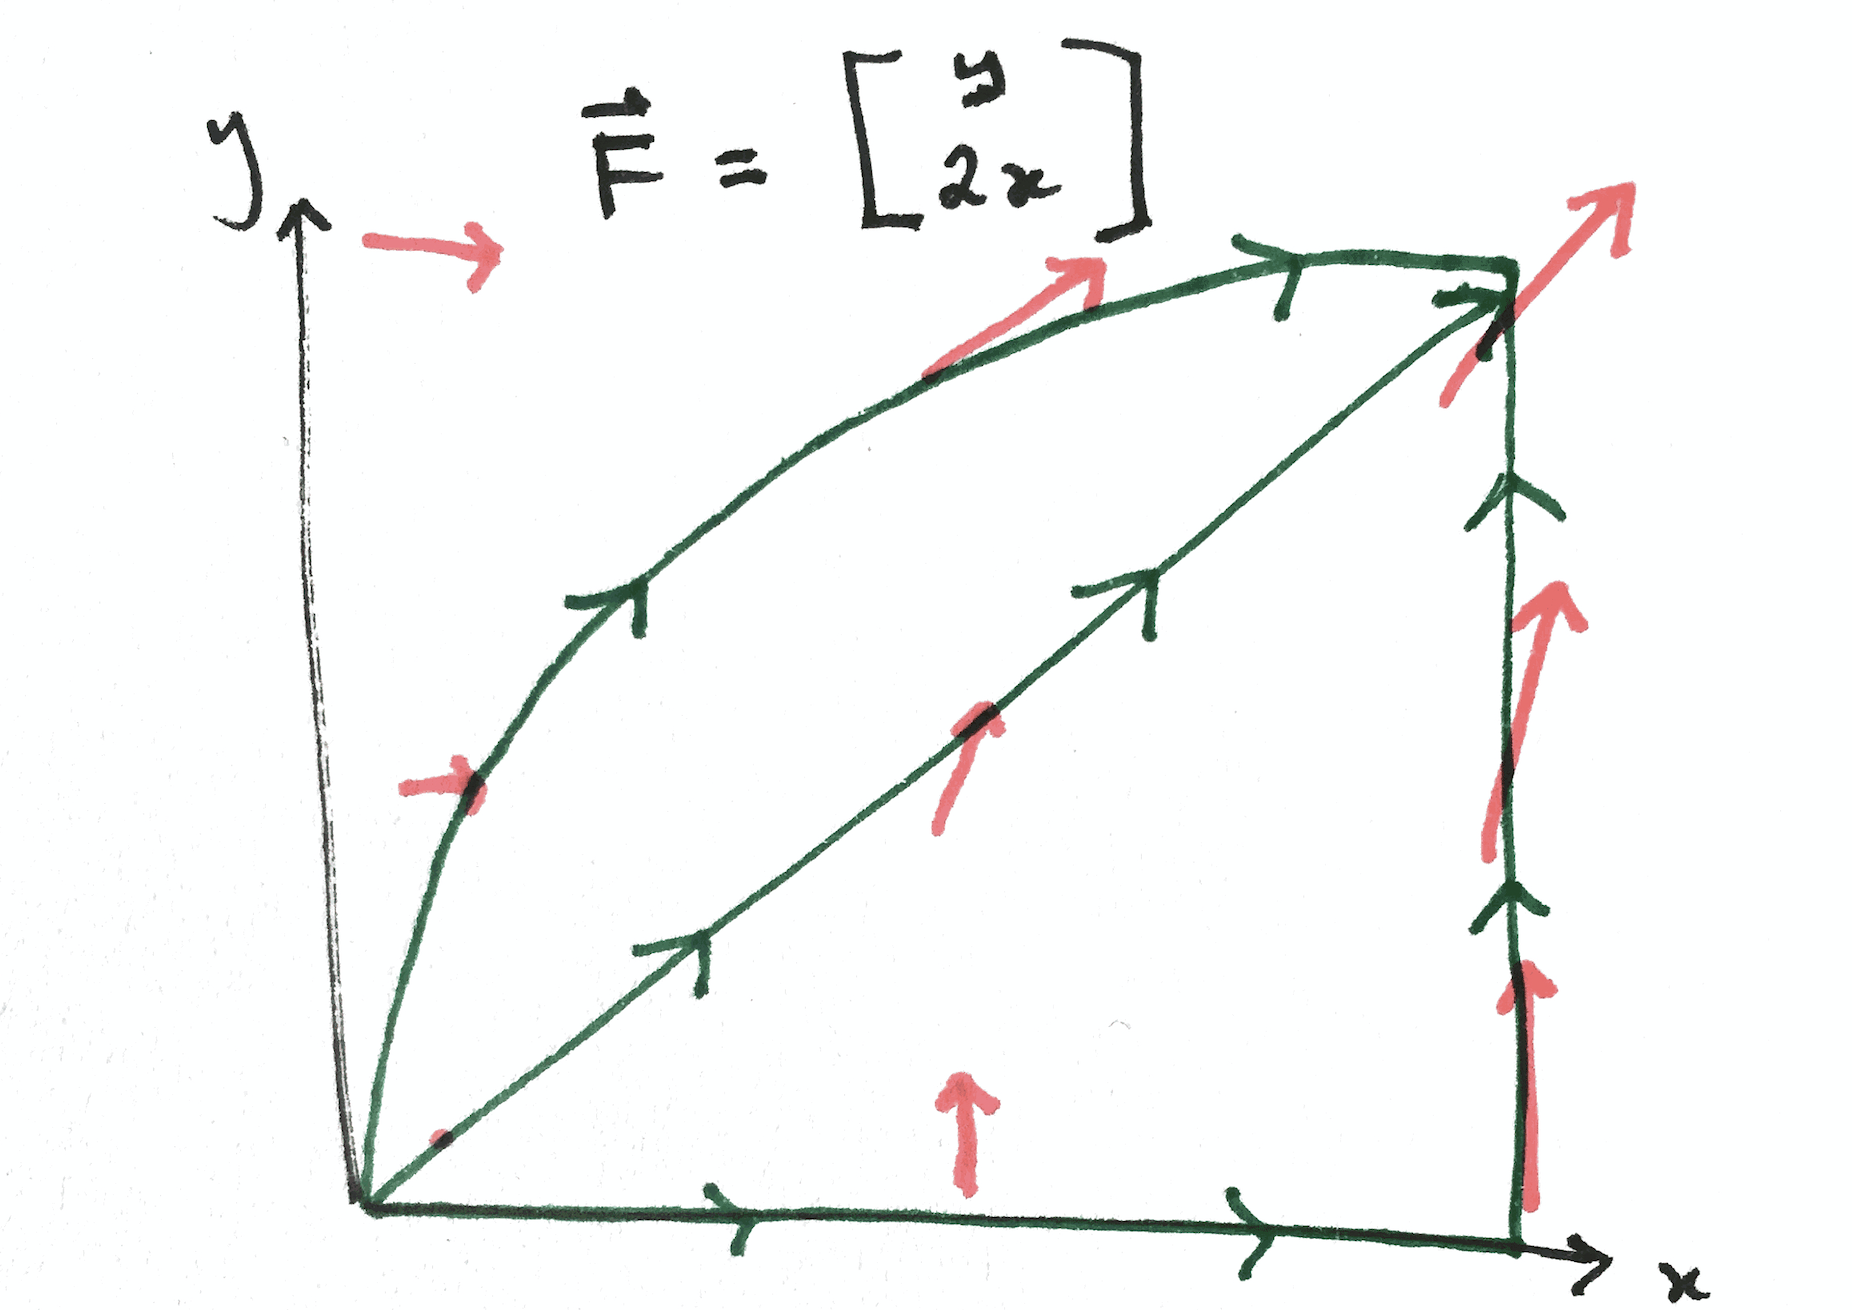
\includegraphics[width=200pt]{img/physics--classical-mechanics--taylor--ex-4-1-diag-2.png}
\end{mdframed}
Qualitatively, we expect the work along (a) to be more than along (b), because (a) coincides with
strong upwards force components on the QP segment. I think work along (c) will be less than (a), but
not sure about (b) vs (c).

\begin{enumerate}[label=(\alph*)]
\item
\begin{align*}
  W
  &= \int_O^Q \F(\r) \cdot \d\r + \int_Q^P \F(\r) \cdot \d\r \\
  &= \int_0^1 F_x(x, 0) \dx + \int_0^1 F_y(1, y) \dy \\
  &= \int_0^1 0 \dx + \int_0^1 2 \dy \\
  &= 2. ~~~ \red{\checkmark}
\end{align*}
\item Along path b we have $y = x$ and therefore $\dy = \dx$.
\begin{align*}
  W
  &= \int_O^P \F(\r) \cdot \d\r \\
  &= \int_O^P F_x(x, y) \dx + F_y(x, y) \dy \\
  &= \int_0^1 F_x(x, x) \dx + F_y(x, x) \dx \\
  &= \int_0^1 x \dx + 2x \dx \\
  &= \frac{3}{2}x^2\Big|_0^1 \\
  &= \frac{3}{2}. ~~~ \red{\checkmark}
\end{align*}
\item For path c, we express the path parametrically:
\begin{align*}
  \r(t)      &= \vecMM{1}{0} + \vecMM{-\cos t}{\sin t}
              = \vecMM{1 - \cos t}{\sin t} \\
  \dot{\r}(t) = \frac{\d\r}{\dt} &= \vecMM{\sin t}{\cos t},
\end{align*}
thus
\begin{align*}
  W
  &= \int_O^P \F(\r) \cdot \d\r \\
  &= \int_O^P \F(\r(t)) \cdot \frac{\d\r}{\dt} \dt \\
  &= \int_0^{\pi/2} \vecMM{\sin t}{2 - 2\cos t} \cdot \vecMM{\sin t}{\cos t} \dt \\
  &= \int_0^{\pi/2} \sin^2 t + 2\cos t - 2\cos^2t \dt \\
  &= \int_0^{\pi/2} 1 - 3\cos^2t \dt + 2\int_0^{\pi/2} \cos t.
\end{align*}
Recall that $\cos 2\theta = \cos^2\theta - \sin^2\theta = 2\cos^2\theta - 1$, therefore
$\cos^2\theta = \frac{1}{2}(1 + \cos 2\theta)$, and therefore
$\int\cos^2\theta \d\theta = \frac{\theta}{2} + \frac{1}{4}\sin 2\theta + C$. So,
\begin{align*}
  W
  &= \Bigg[t - 3\(\frac{t}{2} + \frac{1}{4}\sin 2 t\) + 2\sin t \Bigg]_0^{\pi/2} \\
  &= 2 - \frac{\pi}{4}. ~~~ \red{\checkmark}
\end{align*}

\begin{verbatim}
#+begin_src mathematica :output raw pp
Integrate[Sin[t]^2 + 2 Cos[t] (1 - Cos[t]), t]
#+end_src

#+RESULTS:
: -t/2 + 2*Sin[t] - (3*Sin[2*t])/4

\end{verbatim}




\end{enumerate}

\subsection{4.1}
\begin{mdframed}
  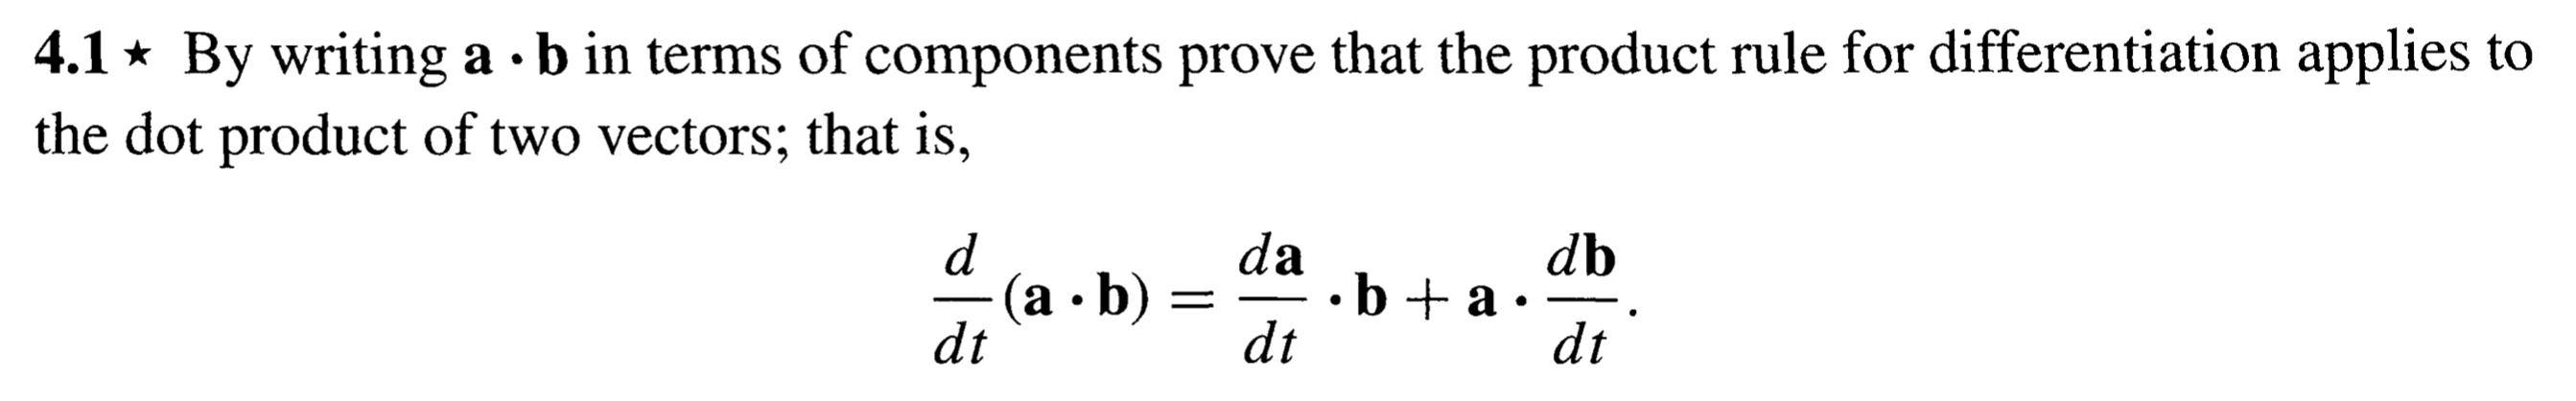
\includegraphics[width=400pt]{img/physics--classical-mechanics--taylor--q-4-1.png}
\end{mdframed}

\begin{align*}
  \ddt (\a \cdot \b)
  &= \ddt \sum a_ib_i \\
  &= \sum \ddt a_ib_i \\
  &= \sum \(\dot{a}_ib_i + a_i\dot{b}_i\) \\
  &= \sum \dot{a}_ib_i + \sum a_i\dot{b}_i \\
  &= \dot{\a} \cdot \b + \a \cdot \dot{\b}.
\end{align*}

\subsection{4.2, 4.3}
\begin{mdframed}
  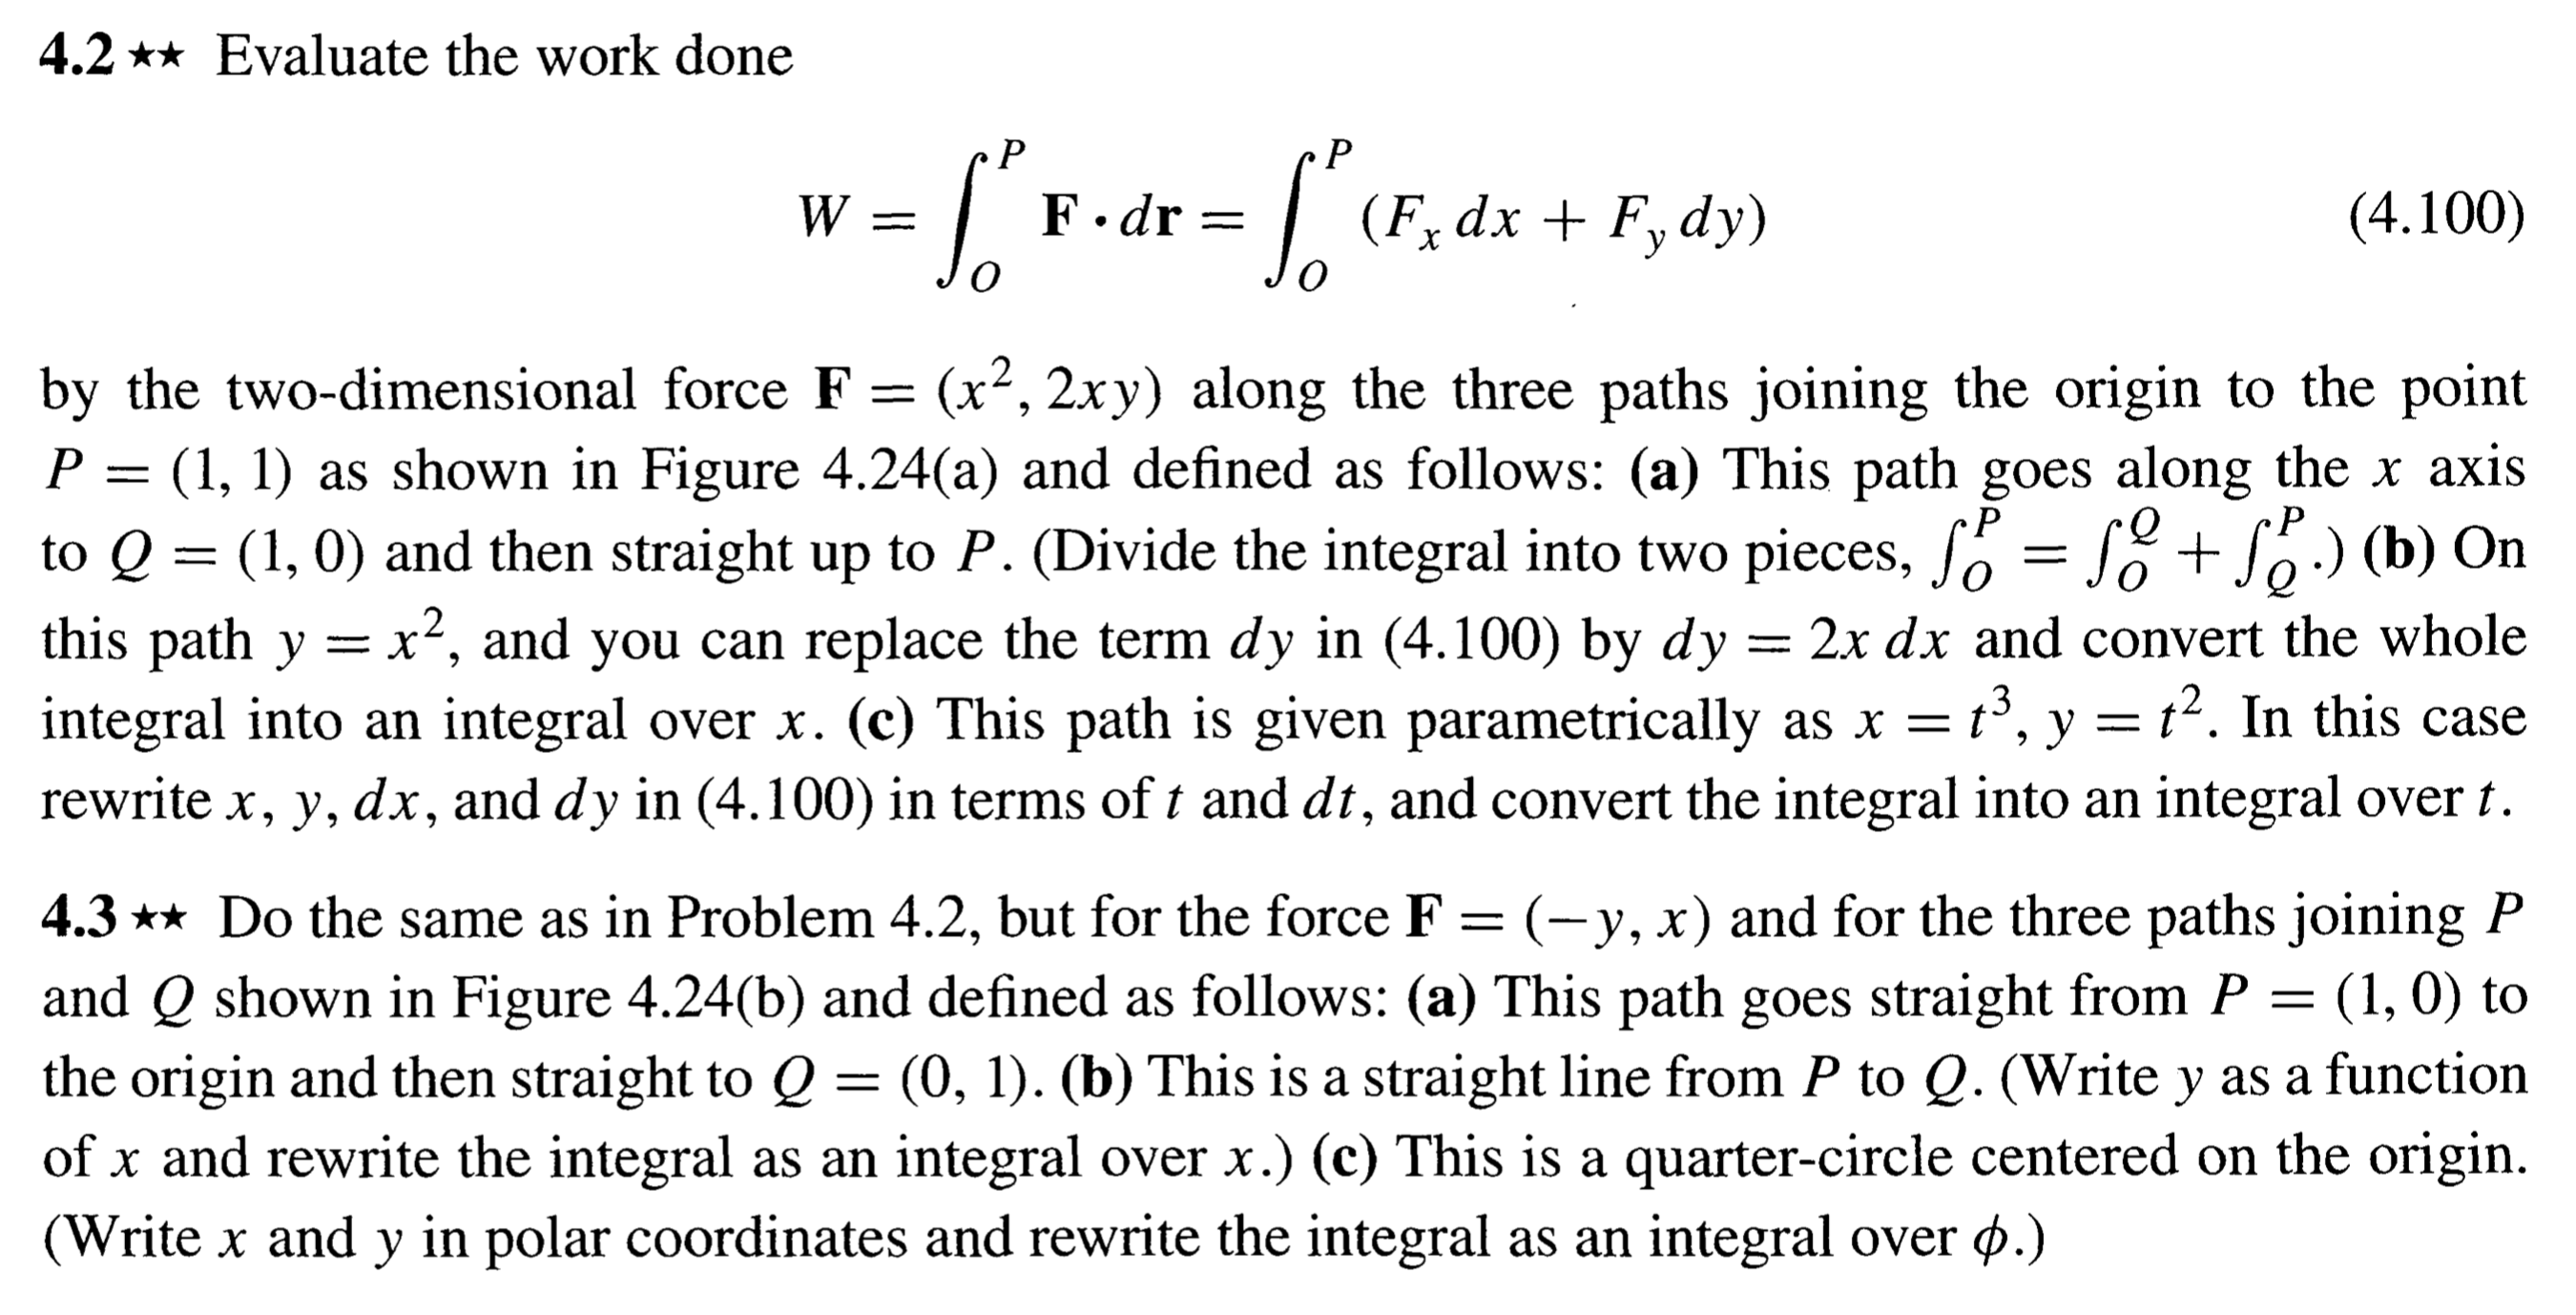
\includegraphics[width=400pt]{img/physics--classical-mechanics--taylor--q-4-3.png}\\
  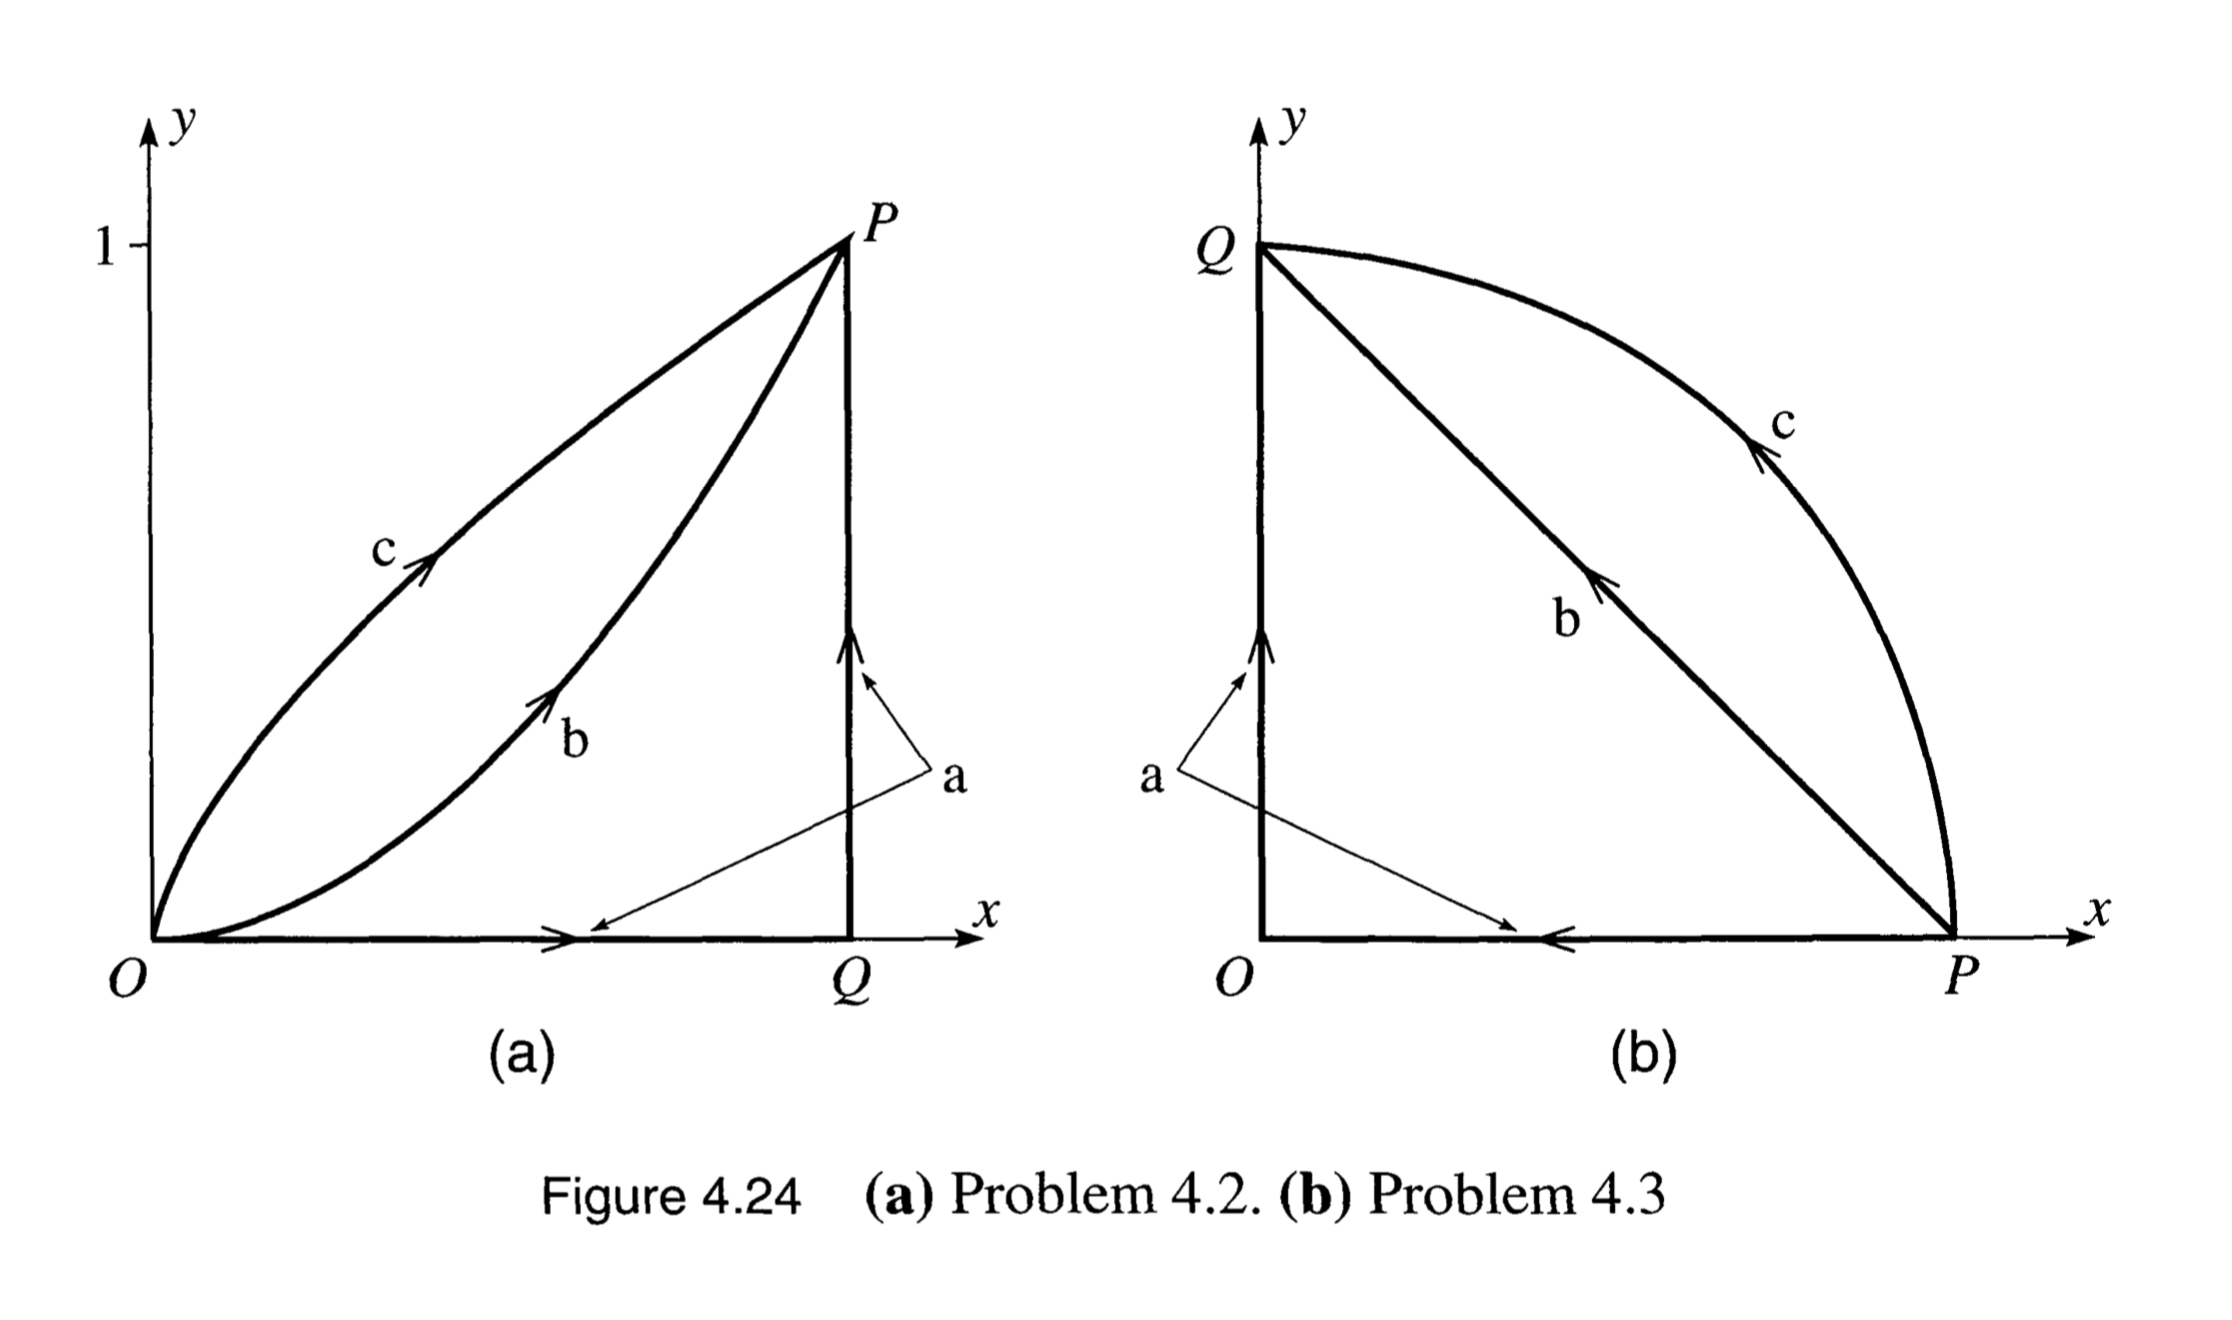
\includegraphics[width=200pt]{img/physics--classical-mechanics--taylor--q-4-3-diag.png}
\end{mdframed}

\begin{enumerate}[label=(\alph*)]
\item Along the segment $PO$ we have $\F \cdot \d\r = 0$ since $F = (0, x)$ and $\d\r = (-\dx,
  0)$. And along the segment $OQ$ we have $\F \cdot \d\r = 0$ since $F = (-y, 0)$ and
  $\d\r = (0, y)$. So the path is perpendicular to the force at all times and hence the work is
  zero:
  \begin{align*}
    W
    &= \int_P^Q \F \cdot \d\r \\
    &= \int_P^O \F \cdot \d\r + \int_O^Q \F \cdot \d\r \\
    &= 0 + 0 = 0. ~~~\red{\checkmark}
  \end{align*}
\item Along $PQ$ we have $y = 1 - x$ and so $\dr = (-\dx, -\dx)$, Therefore
  \begin{align*}
    \int_P^Q \F \cdot \d\r
    &= \int_P^Q F_x(x, y)\dx + F_y(x, y)\dy \\
    &= \int_1^0 -(1-x)\dx + x(-\dx) \\
    &= -\int_1^0 1 \dx \\
    &= 1. ~~~\red{\checkmark}
  \end{align*}
\item The path (c) can be parameterized as
  \begin{align*}
    \r(\phi)            &= \vecMM{\cos \phi}{\sin \phi} \\
    \frac{\d\r}{\d\phi} &= \vecMM{-\sin\phi}{\cos\phi}
  \end{align*}
  for $\phi \in (0, \pi/2)$. Therefore
  \begin{align*}
    W
    &= \int_P^Q \F(\r) \cdot \d\r \\
    &= \int_0^{\pi/2} \F(\r(\phi)) \cdot \frac{\d\r}{\d\phi} \d\phi \\
    &= \int_0^{\pi/2} \vecMM{-\sin\phi}{\cos\phi} \cdot \vecMM{-\sin\phi}{\cos\phi} \d\phi \\
    &= \int_0^{\pi/2} 1 \d\phi \\
    &= \frac{\pi}{2}. ~~~\red{\checkmark}
  \end{align*}
\end{enumerate}
\subsection{4.7}
\begin{mdframed}
  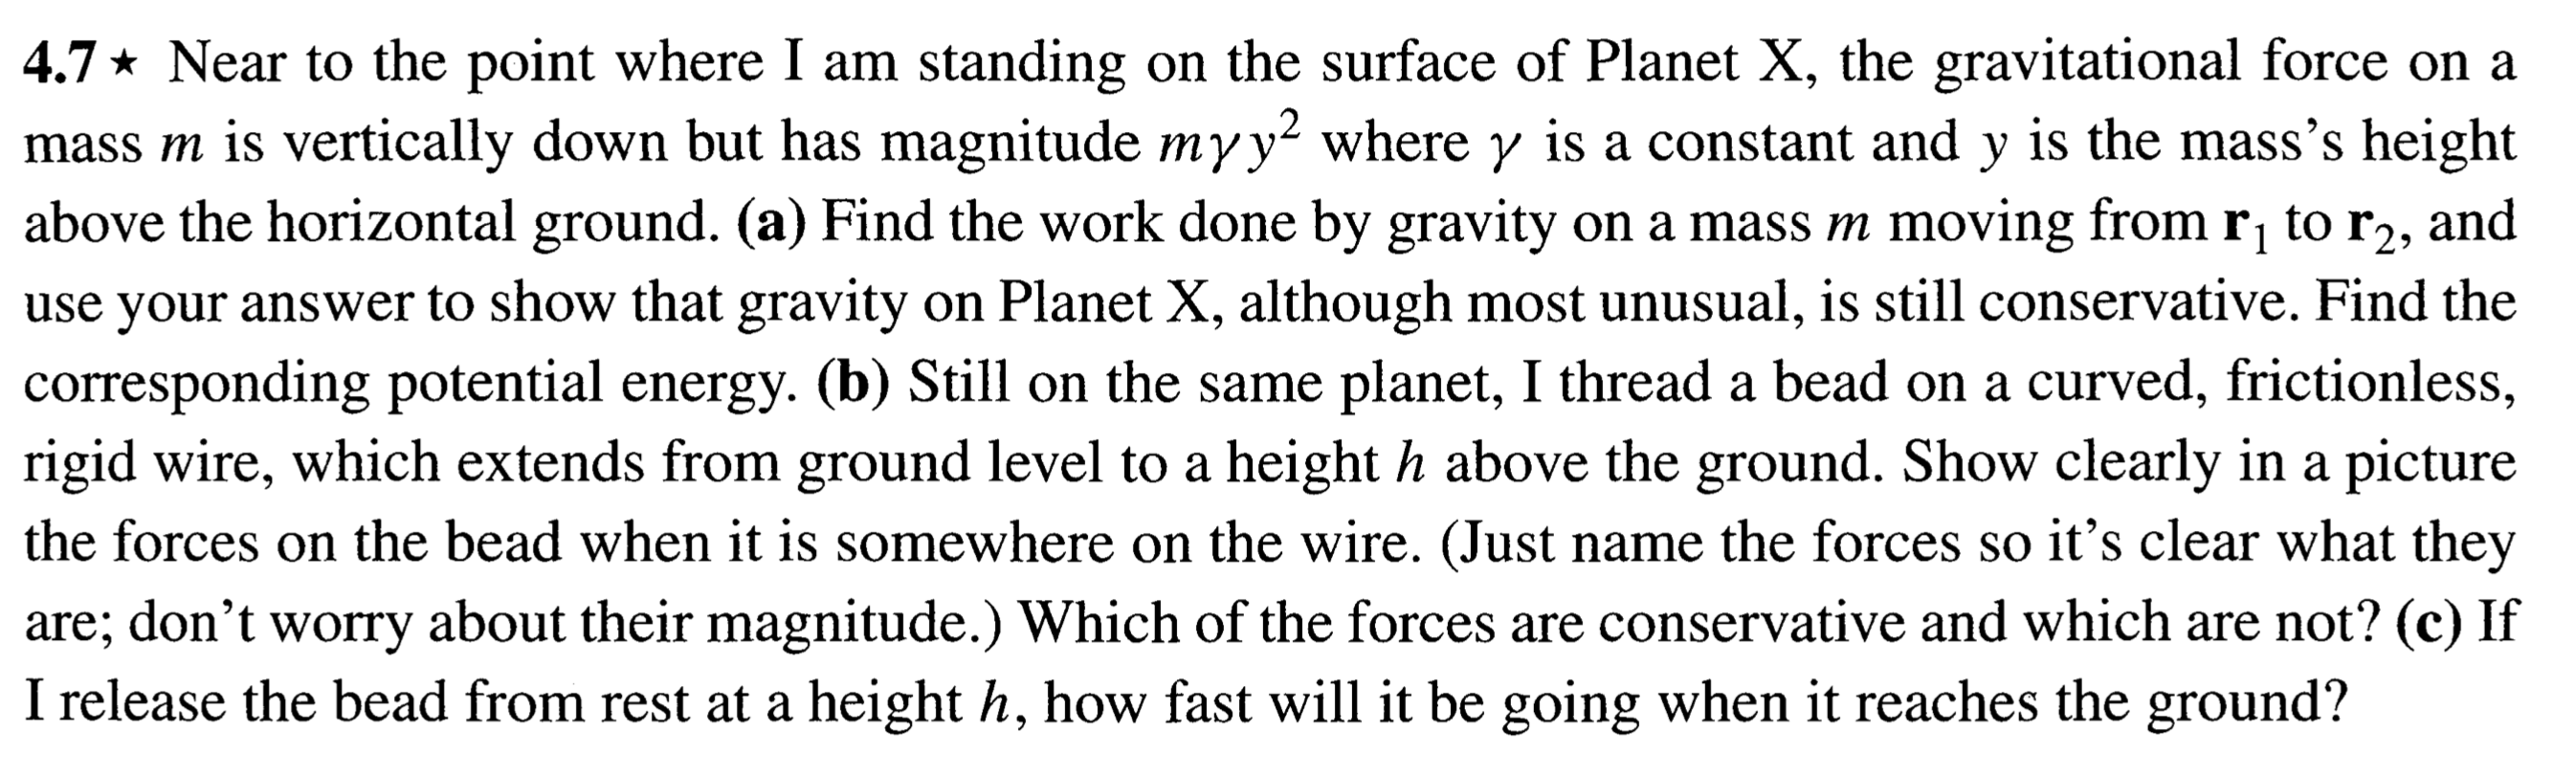
\includegraphics[width=400pt]{img/physics--classical-mechanics--taylor--q-4-7.png}
\end{mdframed}
\begin{enumerate}[label=(\alph*)]
\item Let $x_1$ and $x_2$ measure two horizontal directions, and $y$ measure vertical height.
  \begin{align*}
    W(\r_1 \to \r_2)
    &= \int_{\r_1}^{\r_2} \F(\r) \cdot \d\r \\
    &= \int_{\r_1}^{\r_2} F_{x_1}(x_1, x_2, y)\dx_1 + F_{x_2}(x_1, x_2, y)\dx_2 + F_y(x_1, x_2, y)\dy \\
    &= \int_{y_1}^{y_2} F_y(x_1, yx_2, x)\dy \\
    &= \int_{y_1}^{y_2} -m\gamma y^2\dy \\
    &= -\frac{m\gamma}{3}\(y_2^3 - y_1^3\). ~~~\red{\checkmark}
  \end{align*}
  This depends on the endpoints only and not otherwise on the path, so the force is conservative.
  The potential energy is $V(y) = \frac{m\gamma}{3}y^3$.
\item Conservation of KE + PE at $y=h$ and $y=0$ yields
  \begin{align*}
    0 + \frac{m\gamma}{3}h^3 &= \frac{1}{2}mv^2 + 0 \\
    v &= \sqrt{\frac{2\gamma h^3}{3}}. ~~~\red{\checkmark}
  \end{align*}
\end{enumerate}
\subsection{4.9}
\begin{mdframed}
  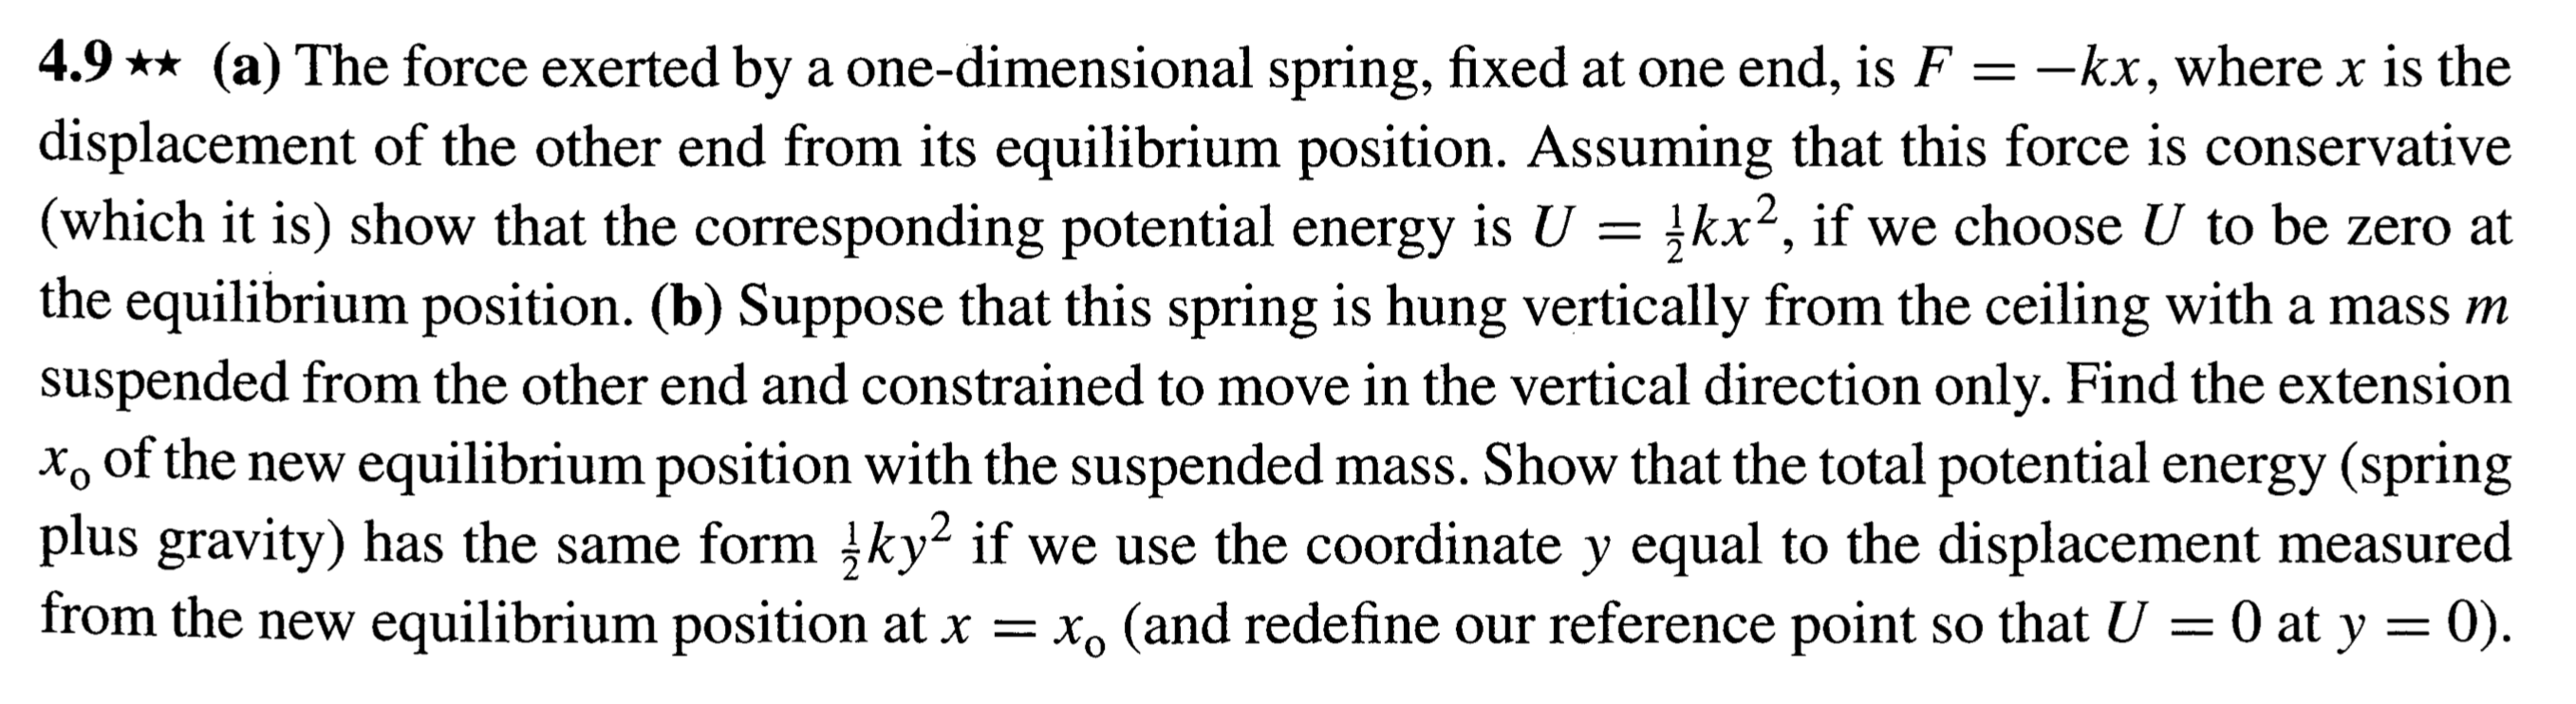
\includegraphics[width=400pt]{img/physics--classical-mechanics--taylor--q-4-9.png}
\end{mdframed}
\begin{enumerate}[label=(\alph*)]
\item
\begin{align*}
  U(x)
  = -\int_0^x F(x) \dx
  = \int_0^x kx \dx = \frac{1}{2}kx^2.
\end{align*}
\item At the new equilibrium we have $mg - kx = 0$ therefore the new equilibrium position is
  $\frac{mg}{k}$ beyond the old equilibrium position. \correct

  Measuring with $y = 0$ at the new equilibrium the potential energy is $U(y) = -\int_0^y (-ky) \dy$ as before.
\end{enumerate}

\subsection{4.11}
\begin{mdframed}
  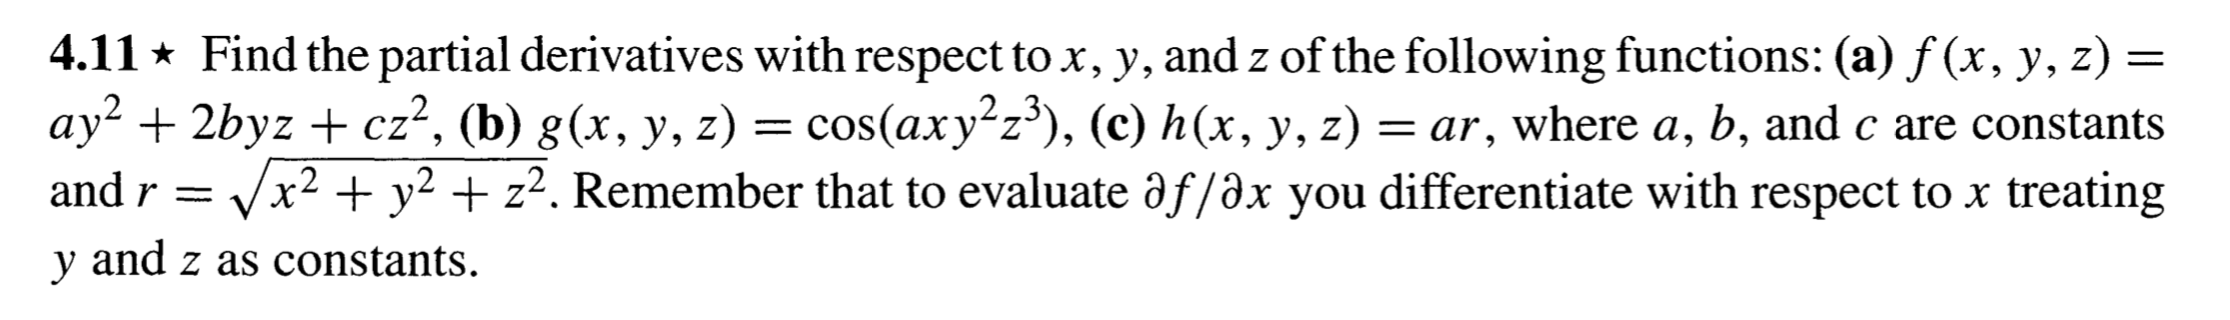
\includegraphics[width=400pt]{img/physics--classical-mechanics--taylor--q-4-11.png}
\end{mdframed}
\begin{enumerate}[label=(\alph*)]
\item
\begin{align*}
  f_x &= 0 \\
  f_y &= 2ay + 2bz \\
  f_z &= 2by + 2cz ~~~\correct
\end{align*}
\item
\begin{align*}
  g_x &= -ay^2z^3\sin(axy^2z^3) \\
  g_y &= -2axyz^3\sin(axy^2z^3) \\
  g_z &= -3axy^2z^2\sin(axy^2z^3) ~~~\correct
\end{align*}
\item
\begin{align*}
  h_x &= ax/r \\
  h_y &= ay/r \\
  h_z &= az/r. ~~~\correct
\end{align*}

\begin{verbatim}
#+begin_src mathematica
D[a Sqrt[x^2 + y^2 + z^2], x]
#+end_src

#+RESULTS:
: (a*x)/Sqrt[x^2 + y^2 + z^2]

\end{verbatim}
\end{enumerate}

\subsection{4.13}
\begin{mdframed}
  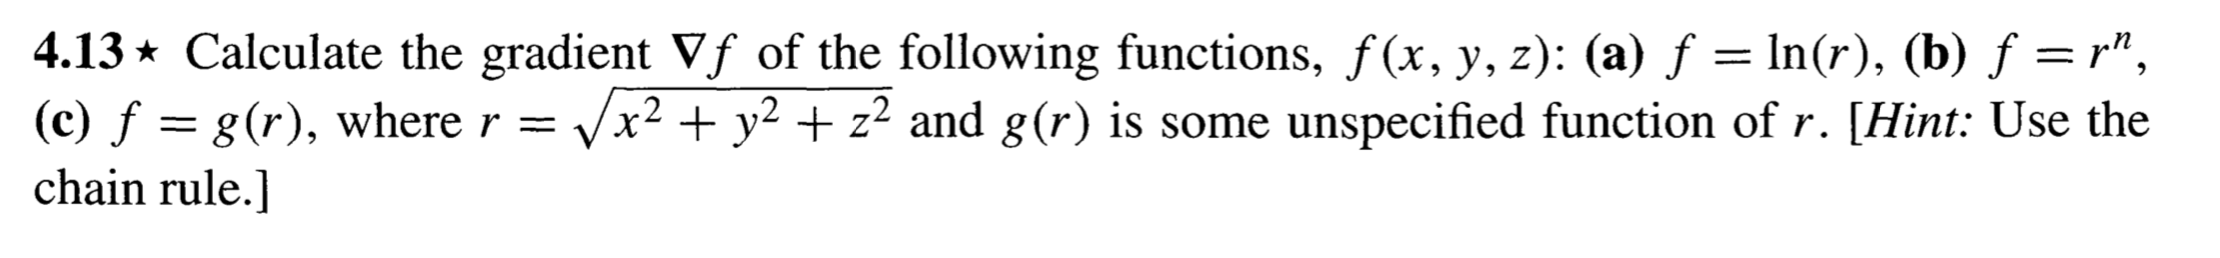
\includegraphics[width=400pt]{img/physics--classical-mechanics--taylor--q-4-13.png}
\end{mdframed}
\begin{enumerate}[label=(\alph*)]
\item $r = (x^2 + y^2 + z^2)^{1/2}$.
  \begin{align*}
    f &= \ln r \\
    \grad f &= \vecMMM{r^{-1}\frac{1}{2}r^{-1}2x}
                      {r^{-1}\frac{1}{2}r^{-1}2y}
                      {r^{-1}\frac{1}{2}r^{-1}2z}
    = \vecMMM{xr^{-2}}{yr^{-2}}{zr^{-2}}
  \end{align*}
\begin{verbatim}
#+begin_src mathematica
D[Log[Sqrt[x^2 + y^2 + z^2]], x]
#+end_src

#+RESULTS:
: x/(x^2 + y^2 + z^2)
\end{verbatim}
\item
\begin{align*}
  \grad r^n
  &= \vecMMM{nxrn^{-2}}{nyrn^{-2}}{nzrn^{-2}}
\end{align*}
\item
  \begin{align*}
    \grad g(r) = \vecMMM{g'(r)x/r}{g'(r)y/r}{g'(r)z/r} ~~~\correct
  \end{align*}
\end{enumerate}

\subsection{4.18}
\begin{mdframed}
  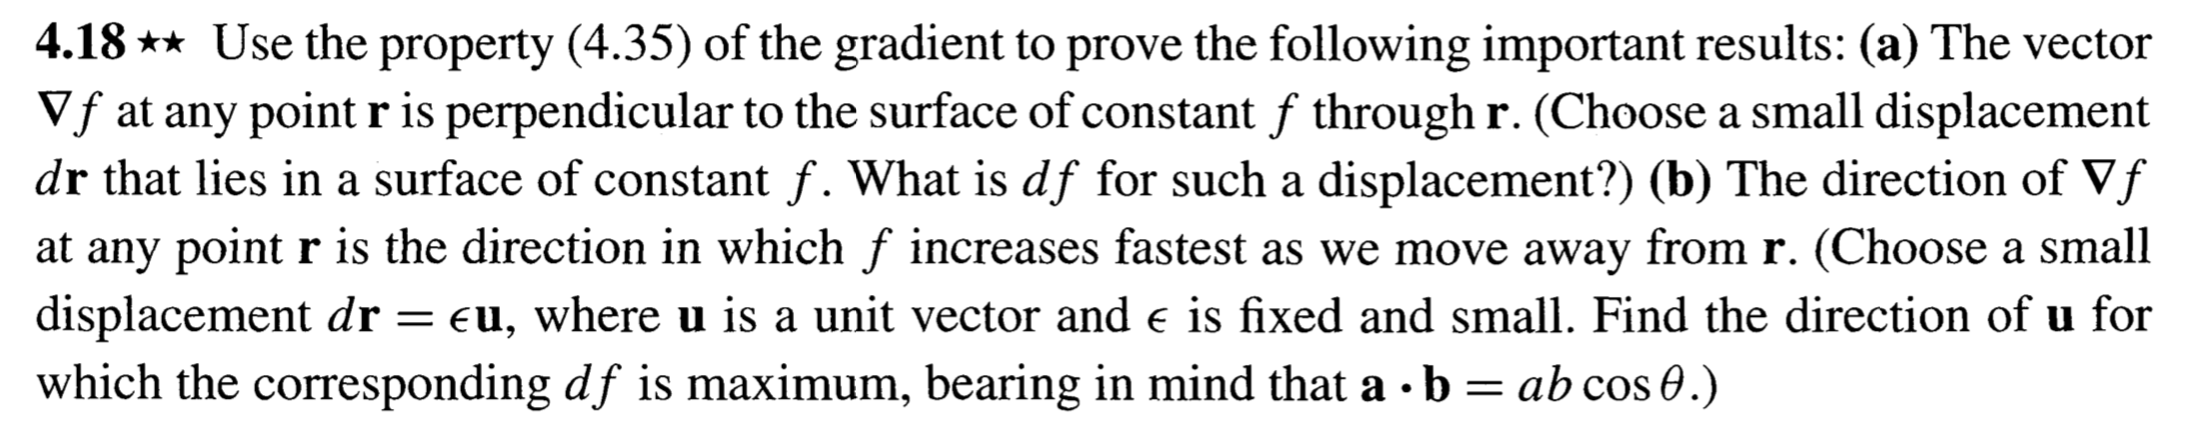
\includegraphics[width=400pt]{img/physics--classical-mechanics--taylor--q-4-18.png}
\end{mdframed}
Property 4.35 is
\begin{align*}
  \df = \grad f \cdot \d\r.
\end{align*}
Intuitively this says that, for a small displacement $\d\r$, the resulting $\df$ is equal to the
projection of a vector $\grad f$ onto $\d\r$. So, if $\d\r$ points in a direction of constant $f$,
then the projection of $\grad f$ onto that $\d\r$ is zero. This is the same as saying that $\grad f$
is perpendicular to such a $\d\r$.

\begin{enumerate}[label=(\alph*)]
\item
  \begin{claim*}
    Let $f:\R^3 \to \R$, and let $\r \in \R^3$. The vector $\grad f$ at $\r$ is perpendicular to the
    surface\footnote{Note that for $f:\R^3 \to \R$, if $f$ is ``nice'', then the level sets of $f$
      form a surface of constant $f$ -- a sort of 2D ``shell'' embedded in $\R^3$.} of constant $f$
    through $\r$.
  \end{claim*}
  \begin{proof}
    Let $\d\r$ lie in a surface of constant $f$. Therefore $\df = f(\r + \d\r) - f(\r) =
    0$. Therefore $\grad f \cdot \d\r = 0$. Therefore these vectors are perpendicular.
  \end{proof}
\item
  \begin{claim*}
    The direction of $\grad f$ at any point $\r$ is the direction in which $f$ increases most
    rapidly as we move away from $\r$.
  \end{claim*}
  \begin{proof}
    Let:
    \begin{itemize}
    \item $f:\R^3 \to \R$
    \item $\r \in \R^3$
    \item $\vec u \in \R^3$ and $|\vec u| = 1$
    \item $\epsilon > 0$
    \item $\d\r = \epsilon\vec u$
    \item $\theta$ be the angle between $(\grad f)(\r)$ and $\vec u$
    \end{itemize}
    The claim is that, out of all possible choices of $\vec u$, the one for which the associated
    $\d\r$ results in the largest $\df$ is the $\vec u$ that points in the same direction as
    $\grad f$.

    We have
    \begin{align*}
      \df
      &= \grad f \cdot \d\r \\
      &= |\grad f| ~ |\d\r| \cos \theta \\
      &= |\grad f|\epsilon \cos \theta \\
    \end{align*}

  \end{proof}
\end{enumerate}

\subsection{4.19}
\begin{mdframed}
  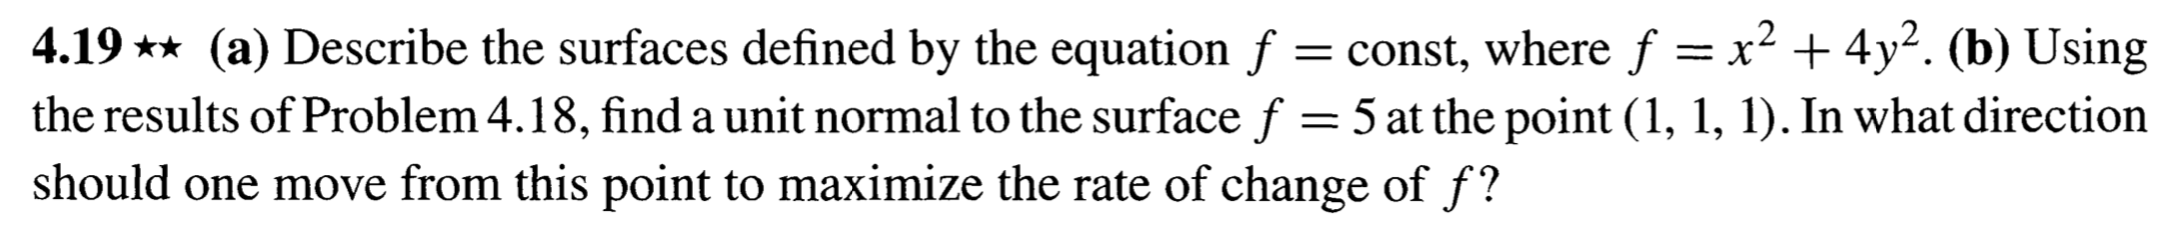
\includegraphics[width=400pt]{img/physics--classical-mechanics--taylor--q-4-19.png}
\end{mdframed}
\begin{enumerate}[label=(\alph*)]
\item The equation $x^2 + 4y^2 = K$ describes an ``elliptical cylinder''
  in $\R^3$. It has radius $\sqrt{K}$ in the $x$-direction and radius
  $\sqrt{K}/2$ in the $y$-direction, and is constant in the $z$
  direction. \correct
\item We have $\grad f = \(2x, 8y, 0\)$. Therefore at the point
  $\r = (1, 1, 1)^T$, we have $(\grad f)(\r) = (2, 8, 0)$. Therefore a
  unit normal is
  $\frac{1}{\sqrt{68}}(2, 8, 0)^T = \sqrt{\frac{1}{17}}(1, 4, 0)^T$,
  and this is also the direction that maximizes change in $f$. \correct
\end{enumerate}
\subsection{4.21}

\begin{definition*}
  The work done by a force $\F$ when it moves a mass along a path
  $\r_1 \to \r_2$ is
\begin{align*}
  W(\r_1 \to \r_2) = \int_{\r_1 \to \r_2} \F(\r) \cdot \d\r.
\end{align*}
\end{definition*}

\begin{definition*}
  A \defn{trajectory} is a function $\r(t)$.
\end{definition*}

\begin{definition*}
  A force is conservative if the work done when it moves a body from $\r_1$ to $\r_2$ is the same for
  all trajectories from $\r_1$ to $\r_2$ that obey Newton's second law.
\end{definition*}

(Note that different initial conditions at $\r_1$ may yield more than one such path.)

\begin{mdframed}
  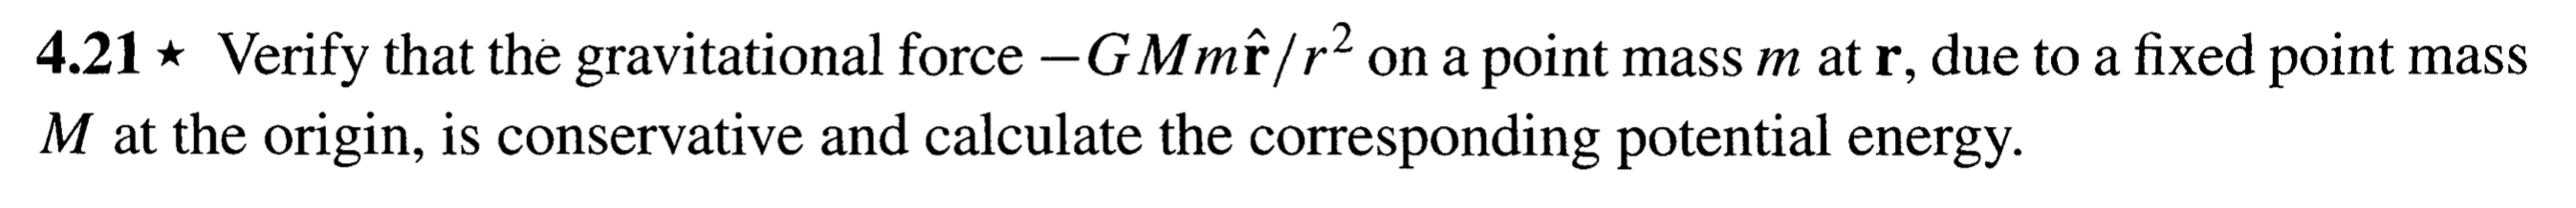
\includegraphics[width=400pt]{img/physics--classical-mechanics--taylor--q-4-21.png}
\end{mdframed}

\begin{proof}
  Let the path be $\r(t)$ where $\r(0) = \r_1$ and $\r(1) = \r_2$, and let $\v(t) = \dot{\r}(t)$. Then
  \begin{align*}
    W(\r_1 \to \r_2) = \int_0^1 \F(\r(t)) \cdot \d\r(t).
  \end{align*}
  Note that
  \begin{enumerate}
  \item since the trajectory obeys Newton's Second Law, we have $\F(\r(t)) = m\ddot{\r}(t) = m\dot{\v}(t)$,
  \item we can write $\d\r = \dot{\r} \dt = \v \dt$,
  \end{enumerate}
  Thus we have
\begin{align*}
  W(\r_1 \to \r_2) &= \int_0^1 m\dot{\v}(t) \cdot \v(t) \dt.
\end{align*}
Note that $\ddt \frac{1}{2}m(\v \cdot \v) = \frac{1}{2}m(\dot{\v} \cdot \v + \v \cdot \dot{\v}) = m\dot{\v} \cdot \v$, therefore
\begin{align*}
  W(\r_1 \to \r_2) &= \frac{1}{2}m|\v(t)|^2\Bigg|_0^1.
\end{align*}
Since the work depends only on the difference in the magnitudes of the velocities at the start and
end points, the force is conservative.

\todo{But couldn't there be two paths between $\r_1$ and $\r_2$ that obey Newton's second law yet for
  which the difference in KE is different?}

\newpage
\begin{mdframed}
  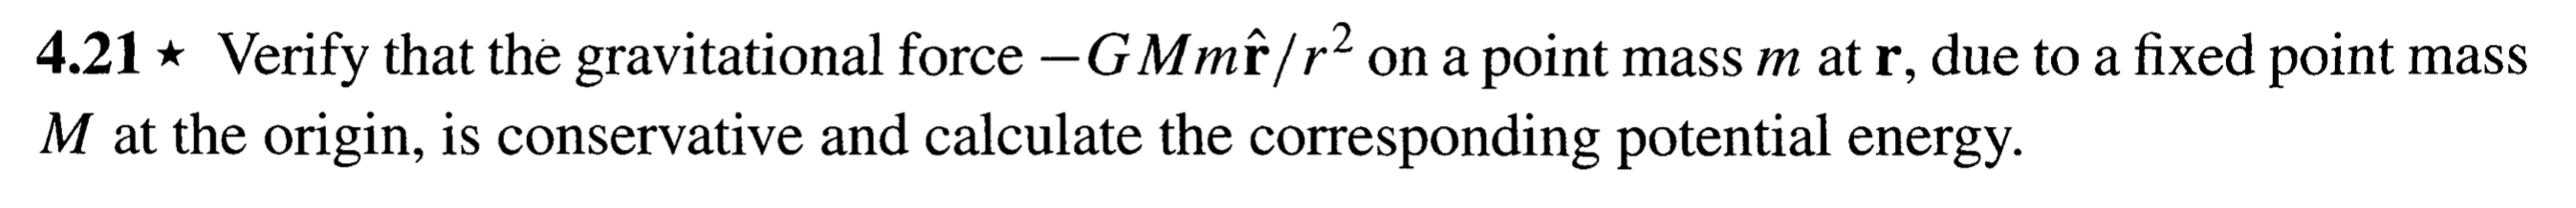
\includegraphics[width=400pt]{img/physics--classical-mechanics--taylor--q-4-21.png}
\end{mdframed}



\begin{mdframed}
  Try again, using the gravitational force:

  The work done by gravity when the mass moves from $\r_1$ to $\r_2$ is
  \begin{align*}
    W(\r_1 \to \r_2) = \int_{\r_1 \to \r_2} \frac{-GMm\hat{\r}}{|\r|^2} \cdot \d\r.
  \end{align*}
  Note that
  \begin{enumerate}
  \item We have $\F(\r(t)) = m\ddot{\r}(t) = m\dot{\v}(t)$,
  \item we can write $\d\r = \dot{\r} \dt = \v \dt$,
  \end{enumerate}
  Thus we have

\end{mdframed}

\end{proof}

% Questions with solutions:

% 3 a,b,c
% 7 a,b,c
% 9 b
% 11
% 13
% 15
% 19 a b
% 21
% 23 a b c
% 29 a b d
% 31 a
% 33 b c
% 35 a b
% 37 a b c d
% 39 c
% 51
% 53 b c
